\subsection{Phân hệ Văn phòng số, Nhiệm vụ và Lịch công tác (iOffice)}
\label{subsec:module_ioffice}
\label{subsec:req_schedule}

\subsubsection{Mục tiêu}
Phân hệ Văn phòng số, Nhiệm vụ và Lịch công tác kết nối trực tiếp với dịch vụ \texttt{ioffice-be} của Nhà trường, cung cấp cho viên chức, giảng viên khả năng tra cứu văn bản đến/đi, theo dõi tiến độ công việc và chủ động theo dõi các sự kiện lịch công tác tuần của Nhà trường và đơn vị trên thiết bị di động.

Đối với các cuộc họp có cấu hình điểm danh, ứng dụng hỗ trợ tính năng điểm danh có mặt hoặc báo vắng kèm lý do giải trình. Mọi điều kiện hợp lệ về thẩm quyền và khung thời gian điểm danh phải được backend kiểm soát độc lập, không phụ thuộc vào đồng hồ thời gian hoặc trạng thái do thiết bị di động tự thiết lập.

\subsubsection{Yêu cầu chức năng}

\begin{itemize}[leftmargin=1.5cm]
    \item \textbf{FR-SCH-01 -- Xem lịch công tác:} Người dùng có quyền phải có khả năng tra cứu danh sách các sự kiện lịch tuần trường, lịch đơn vị và xem thông tin chi tiết: chủ trì, thời gian bắt đầu/kết thúc, địa điểm, thành phần tham dự và nội dung cuộc họp.
    
    \item \textbf{FR-SCH-02 -- Hiển thị thao tác điểm danh:} Đối với các cuộc họp có cấu hình điểm danh, ứng dụng phải tự động hiển thị nút bấm thao tác điểm danh/báo vắng khi sự kiện nằm trong khoảng thời gian cho phép.
    
    \item \textbf{FR-SCH-03 -- Điểm danh có mặt:} Người dùng phải có khả năng gửi yêu cầu ghi nhận có mặt đối với cuộc họp mà mình có tên trong danh sách đại biểu được mời tham dự.
    
    \item \textbf{FR-SCH-04 -- Báo vắng:} Người dùng có thể khai báo vắng mặt và bắt buộc phải cung cấp lý do vắng hợp lệ (độ dài quy định) khi chức năng này được sự kiện cho phép.
    
    \item \textbf{FR-SCH-05 -- Kiểm tra tại backend:} Backend phải thẩm định lại danh tính người dùng, quyền tham dự cuộc họp và điều kiện khung giờ hợp lệ trước khi ghi nhận trạng thái điểm danh vào cơ sở dữ liệu.
    
    \item \textbf{FR-SCH-06 -- Đồng bộ thay đổi:} Khi trạng thái điểm danh của cuộc họp thay đổi, ứng dụng phải cập nhật ngay giao diện hiển thị; các thay đổi phát sinh từ người dùng khác có thể được cập nhật theo thời gian thực qua kênh kết nối mạng của hệ thống.
\end{itemize}

\subsubsection{Đặc tả Ca sử dụng (Use Cases)}

\usecasespec{
  id={UC-SCH-01},
  name={Điểm danh cuộc họp},
  actor={Cán bộ / Giảng viên có tên trong danh sách tham dự cuộc họp.},
  pre={Người dùng đã đăng nhập; cuộc họp được cấu hình hỗ trợ ghi nhận tham dự.},
  trigger={Người dùng mở xem chi tiết cuộc họp trên ứng dụng.},
  mainflow={
    1. Mobile kiểm tra sơ bộ khung giờ diễn ra cuộc họp và hiển thị các tùy chọn điểm danh. \newline
    2. Người dùng nhấn nút \textit{``Điểm danh có mặt''} (hoặc \textit{``Báo vắng''} kèm nhập lý do). \newline
    3. Mobile gửi request lên backend dịch vụ. \newline
    4. Backend kiểm tra tính hợp lệ của phiên, quyền tham dự của cán bộ và thời gian hiện tại trên máy chủ. \newline
    5. Backend ghi nhận trạng thái tham dự vào cơ sở dữ liệu và phát sự kiện đồng bộ. \newline
    6. Mobile nhận phản hồi thành công và cập nhật trạng thái hiển thị trên giao diện sang \textit{``Đã điểm danh''}.
  },
  altflow={
    Cuộc họp chưa đến giờ mở điểm danh, đã kết thúc hoặc cán bộ không thuộc danh sách tham dự $\rightarrow$ Backend từ chối ghi nhận; ứng dụng hiển thị thông báo lỗi tương ứng.
  },
  post={Bản ghi tham dự cuộc họp của cán bộ được lưu trữ chính thức tại hệ thống iOffice.},
  label={tab:uc_sch_01}
}

\usecasespec{
  id={UC-IOFFICE-01},
  name={Tra cứu Văn bản Đến/Đi và Bút phê Phân phối Chỉ đạo},
  actor={Cán bộ xem văn bản, Lãnh đạo Đơn vị (Người chỉ đạo)},
  pre={Cán bộ đã đăng nhập; có quyền truy cập văn phòng điện tử.},
  mainflow={
    1. Cán bộ mở màn hình \texttt{IncomingDocsListPage} hoặc \texttt{OutgoingDocsListPage}. \newline
    2. Hệ thống tải danh sách văn bản phân trang cuộn vô tận (\texttt{InfiniteScrollPagination}). \newline
    3. Nhấn vào một văn bản cụ thể $\rightarrow$ Mở màn hình \texttt{IncomingDocDetailPage}, tích hợp trình đọc PDF (\texttt{pdfrx}) hiển thị nội dung toàn văn. \newline
    4. Lãnh đạo Đơn vị nhấn nút \textit{``Phân phối văn bản''}, chọn cán bộ xử lý chính, cán bộ phối hợp, hạn chót và nhập bút phê chỉ đạo. \newline
    5. Nhấn \textit{``Lưu chỉ đạo''} $\rightarrow$ Hệ thống ghi nhận vào \texttt{van\_ban\_den\_distribution} và phát thông báo đẩy tới các cán bộ được giao việc.
  },
  post={Cán bộ đọc được nội dung văn bản; văn bản được phân phối kèm chỉ đạo xử lý.},
  label={tab:uc_ioffice_01}
}

\usecasespec{
  id={UC-IOFFICE-02},
  name={Quản lý \& Giám sát Tiến độ Nhiệm vụ (Tasks/Missions)},
  actor={Cán bộ thực hiện, Lãnh đạo Đơn vị, Ban Giám hiệu},
  pre={Nhiệm vụ đã được khởi tạo trong hệ thống điều hành của Nhà trường.},
  mainflow={
    1. Người dùng mở \texttt{MissionsListPage}, lọc theo loại nhiệm vụ (Trọng tâm/Được giao/Chung) và 5 trạng thái. \newline
    2. Chọn một nhiệm vụ cụ thể $\rightarrow$ Mở \texttt{MissionDetailPage} với 4 tab (Tổng quan, Cây đầu việc \texttt{outlined-tree}, Báo cáo đợt, Văn bản liên kết). \newline
    3. Nhấn vào một công việc trong cây đầu việc $\rightarrow$ Mở \texttt{TaskDetailBottomSheet} để xem người phụ trách và checklist. \newline
    4. Cán bộ nhấn \textit{``Nộp báo cáo đợt''}, nhập nội dung, \% tiến độ hoàn thành và đính kèm tài liệu minh chứng $\rightarrow$ Nhấn gửi. \newline
    5. Hệ thống lưu vào bảng \texttt{mission\_report\_batch} và cập nhật lại tiến độ tổng thể của nhiệm vụ.
  },
  post={Cán bộ cập nhật tiến độ công việc và gửi báo cáo đợt thành công.},
  label={tab:uc_ioffice_02}
}

\subsubsection{Quy tắc nghiệp vụ (Business Rules)}

\begin{itemize}[leftmargin=1.5cm]
    \item \textbf{BR-SCH-01:} Chỉ các sự kiện lịch họp được nhà trường cấu hình bật tính năng ghi nhận tham dự mới cho phép người dùng thực hiện điểm danh hoặc báo vắng.
    \item \textbf{BR-SCH-02:} Điều kiện thời gian kiểm tra trên thiết bị di động chỉ đóng vai trò hỗ trợ giao diện (UX Gate); thời gian trên máy chủ backend (Server Time) là căn cứ thẩm quyền duy nhất để quyết định tính hợp lệ của thao tác điểm danh.
    \item \textbf{BR-SCH-03:} Người dùng chỉ được phép điểm danh cho các cuộc họp mà tài khoản của họ được phân công tham dự hoặc được mời với tư cách đại biểu hợp lệ.
    \item \textbf{BR-SCH-04:} Khi thực hiện báo vắng, nội dung lý do báo vắng bắt buộc phải thỏa mãn yêu cầu về độ dài và định dạng do backend quy định (ví dụ tối thiểu từ 1 đến 200 ký tự).
    \item \textbf{BR-SCH-05:} Ứng dụng di động không được xem dữ liệu nhận được từ kênh thời gian thực (real-time stream) là nguồn dữ liệu có thẩm quyền thay thế cho trạng thái lưu trữ chính thức trong cơ sở dữ liệu backend.
\end{itemize}

\subsubsection{Biểu đồ Hoạt động (Activity Diagrams)}

\begin{figure}[H]
    \centering
    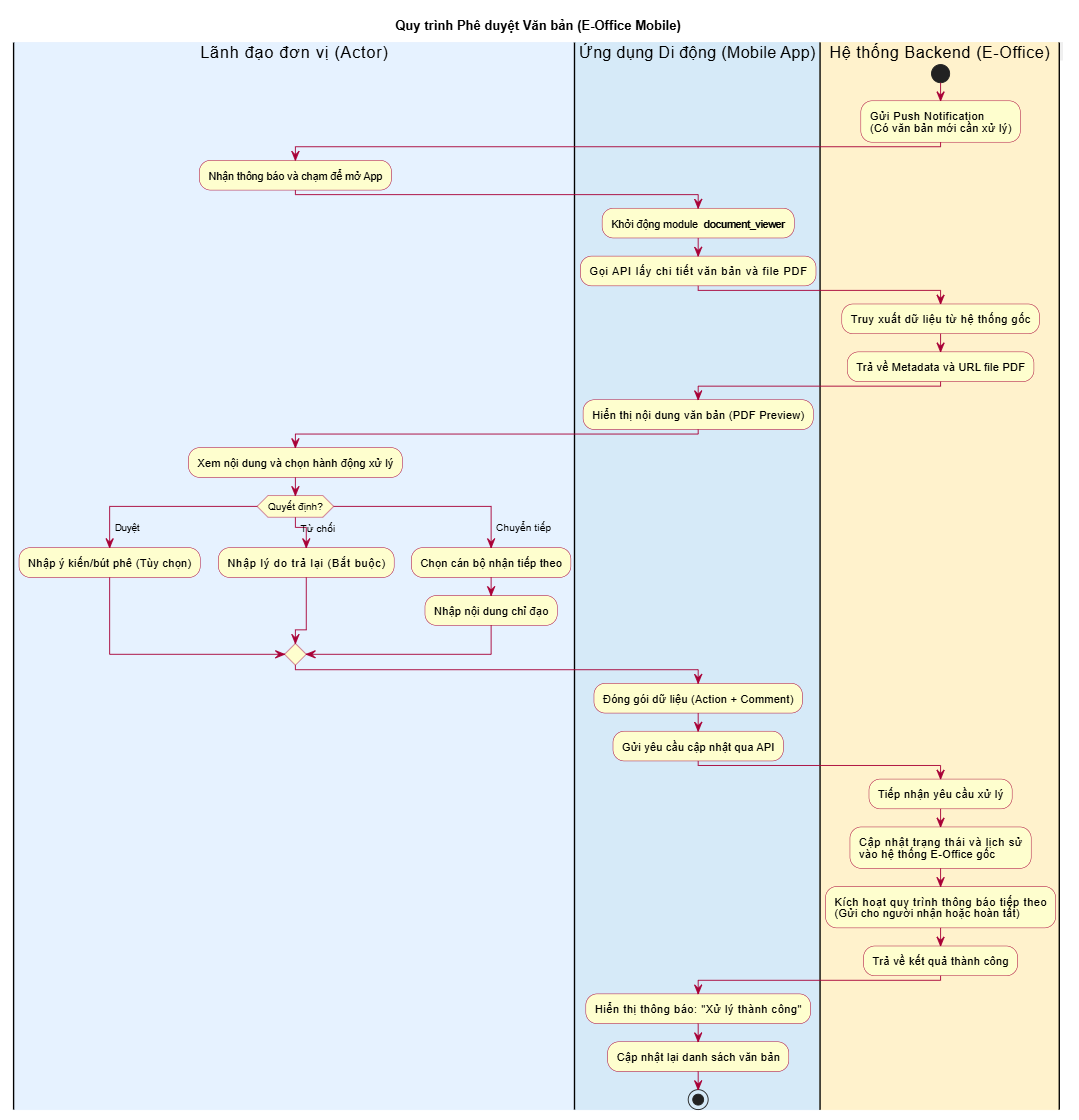
\includegraphics[width=0.85\linewidth]{img/uml/activity_mission_workflow.png}
    \caption{\textit{Biểu đồ Hoạt động Quy trình Quản lý và Theo dõi Tiến độ Nhiệm vụ}}
    \label{fig:act_ioffice_mission}
\end{figure}

\begin{figure}[H]
    \centering
    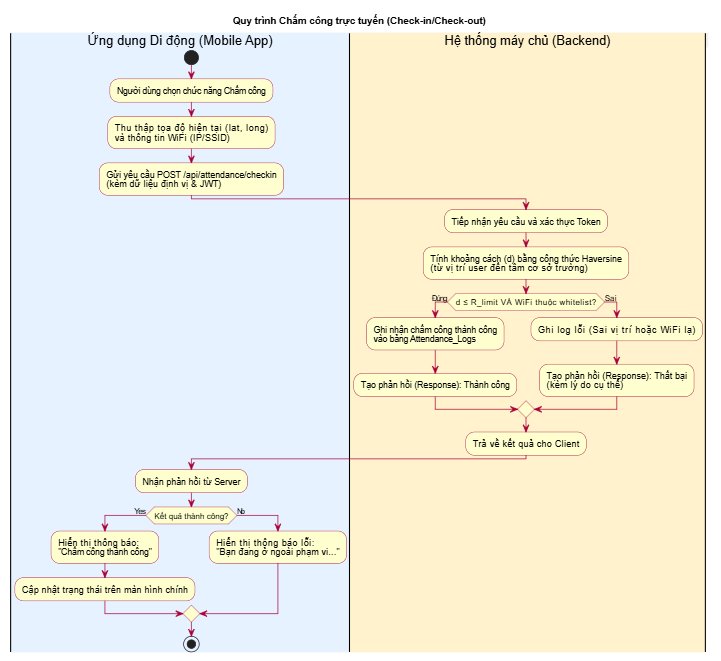
\includegraphics[width=0.85\linewidth]{img/uml/activity_schedule_attendance.png}
    \caption{\textit{Biểu đồ Hoạt động Quy trình Điểm danh Cuộc họp Thời gian thực}}
    \label{fig:act_ioffice_attendance}
\end{figure}

\subsubsection{Biểu đồ Tuần tự (Sequence Diagrams)}

\begin{figure}[H]
    \centering
    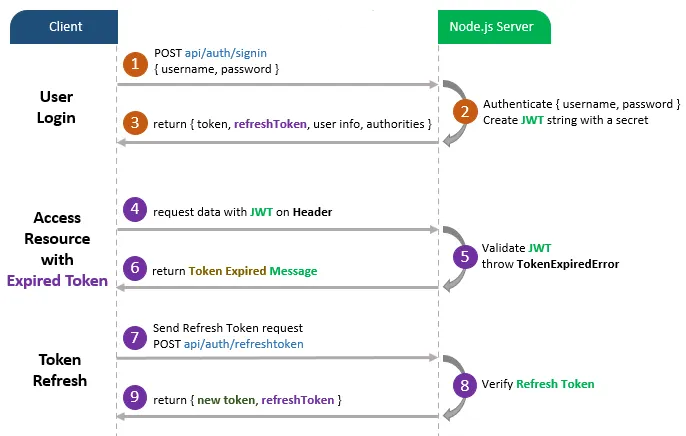
\includegraphics[width=0.85\linewidth]{img/uml/seq_mission_tasks.png}
    \caption{\textit{Biểu đồ Tuần tự Quản lý Nhiệm vụ, Cây Đầu việc và Báo cáo Tiến độ}}
    \label{fig:seq_ioffice_mission}
\end{figure}

\begin{figure}[H]
    \centering
    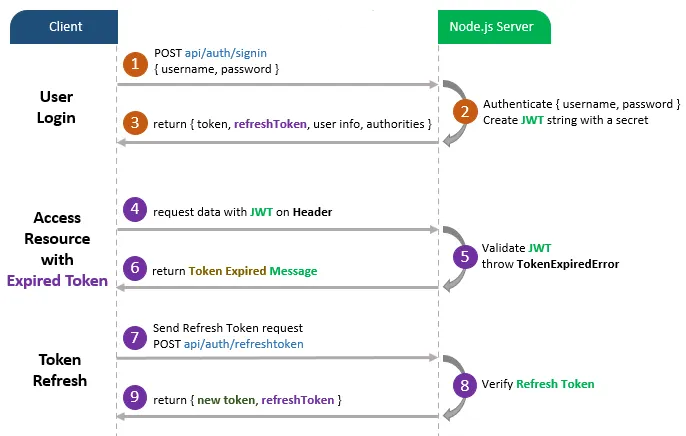
\includegraphics[width=0.85\linewidth]{img/uml/seq_meeting_checkin.png}
    \caption{\textit{Biểu đồ Tuần tự Điểm danh Cuộc họp Thời gian thực qua WebSocket Socket.IO}}
    \label{fig:seq_ioffice_checkin}
\end{figure}
